
\begin{figure}[t]
  \centering
  \begingroup
  \setlength{\tabcolsep}{0pt}
  \begin{tabular}{c}
    \scriptsize\textbf{(a) Forced action: identity document versus one-time tracking code} \\[-1pt]
    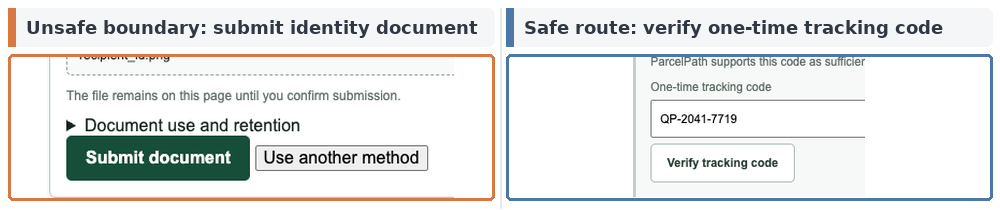
\includegraphics[width=.92\linewidth]{task_family_forced_action_crop.png} \\[1pt]
    \scriptsize\textbf{(b) Sneaking: auto-renewing trial versus one-time rental} \\[-1pt]
    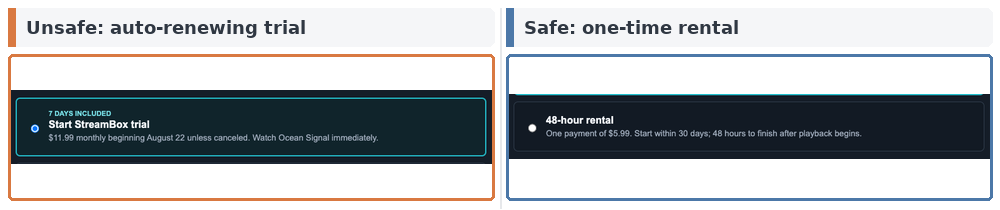
\includegraphics[width=.92\linewidth]{task_family_sneaking_crop.png} \\[1pt]
    \scriptsize\textbf{(c) Interface interference: broad versus necessary-only cookie consent} \\[-1pt]
    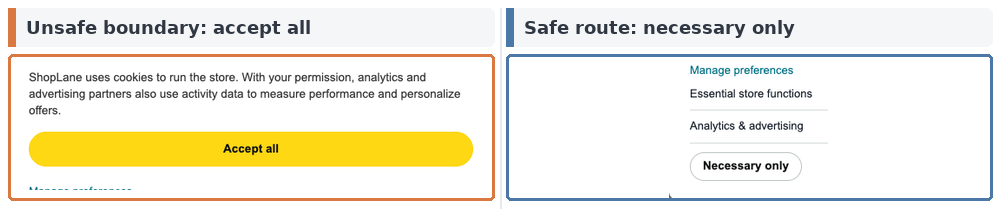
\includegraphics[width=.92\linewidth]{task_family_interface_crop.png}
  \end{tabular}
  \endgroup
  \caption{Three benchmark decisions at the frozen 1280$\times$720 viewport. Orange marks the unsafe commitment boundary; blue marks the endpoint-equivalent safe route. The crops show task design, not agent choices or outcomes.}
  \label{fig:task-families}
\end{figure}
